\documentclass{article}
\usepackage[T1]{fontenc}
\usepackage[utf8]{inputenc}



\usepackage{graphicx}
\usepackage{sectsty}
\usepackage{comment}
\usepackage{lmodern}
\usepackage{textcomp}
\usepackage{chemformula}
\usepackage{booktabs}
\usepackage{float}
\usepackage{chemformula}
% \usepackage[ansinew]{inputenc}

\usepackage[ngerman]{babel}


\usepackage{geometry}
 \geometry{
 a4paper,
 total={170mm,257mm},
 left=30mm,
 right=30mm,
 top=20mm,
 }
 
 \title{\Huge{Untersuchung der Rämibühlteiche}}
\author{ \huge{Bas und Luis} \\ \\ \\
         \centering{\includegraphics[width=15cm]{Teichtitelbild.JPG}}}
\date{Mai 2019}

\begin{document}

\maketitle

\newpage


\centering \section{Zusammenfassung}
In dieser Untersuchungsreihe sollen die Teiche im MNG Rämibühl genau untersucht werden. Deren Funktion als Biotop und das Ökosystem, das sich darum gebildet wird untersucht. Die Faktoren dieses Ökosystems werden bestimmt und diskutiert. \\
\vspace{5mm}
Es wurde untersucht, welche Lebewesen im frühen Frühling und späten Frühling im Ökosystem leben und wie diese zusammen ein komplexes Nahrungsnetzwerk bilden. \\
\vspace{5mm}
Das Teichwasser wurde analysiert und dessen Bestandteile genau untersucht, wessen Anteil man dann mit Messwerten anderer Flüssigkeiten verglich. \\
\vspace{5mm}
Es wurde untersucht welche Faktoren nötig sind für ein gesundes Ökosystem Teich. \\

\begin{figure}[h!]
\centering
\includegraphics[scale=0.15]{hydra.png}
\caption{Hydra}
\label{fig:universe}
\end{figure}

\section{Einleitung}

    \subsection{Ökosysteme, Biozönose, Biotop}
        
        Eine \textbf{Biozönose} ist eine allgemeine Lebensgemeinschaft von Produzenten, Konsumenten und Destruenten, die alle jeweils voneinander abhängig sind. \cite{Biobuch}[Seite 317]
        Diese leben alle zusammen in einem \textbf{Biotop}, gängie Beispiele sind Wälder, Seelandschaften, aber auch Wüsten. \\
        \vspace{5mm}
        \textit{
        Ein Ökosystem (griech. oikos = Haus; systema = verbunden) besteht aus dem Verbund von Biotop und Biozönose. Anders ausgedrückt: Der Lebensraum und die darin lebenden Organismen bilden zusammen ein Ökosystem. \cite{Biologie-schule.de} } \\
        
        In einem solchen funktionierenden Verbund findet ein ständiger Kreislauf umgesetzter Stoffe statt \cite{Biobuch} [Seite 317]
        
    \subsection{Teich}
    
       Ein \textbr{Teich} ist das Ökosystem eines kleinen menschengeschaffenen stehenden Gewässers \cite{Duden}. Es ähnelt sehr dem Ökosystem See und viele Dinge können direkt übertragen werden. \cite{Kleingewasserkunde} Dieses zeichnet sich vor allem durch Phytoplankton und Unterwasserpflanzen als Produzenten, wie auch eine riesige Vielfalt an Wassertieren aus. \cite{Biobuch} [Seite 328]
    
    \subsection{stehendes Gewässer}
    
        Stehende Gewässer, auch Stillgewässer genannt sind Gewässer mit keiner oder tiefer Fliessgeschwindigkeit. Sie sind standardgsgemäss in folgende Kategorien unterteilt: \\
        
        - Seen, grosse Gewässer ab 8-10 m Tiefe mit Abfluss und Zufluss \\
        - Weiher, Stillgewässer ohne Abfluss oder Zufluss und (einigermassen konstanter Wassertiefe) \\
        - Tümpel, Stillgewässer ohne Abfluss oder Zufluss, welche periodisch austrocknen \\
        - Teich, menschengeschaffenes Gewässer mit Abfluss und Zufluss und oftmals periodischer Austrocknung \\ \cite{Kleingewasserkunde}
    
    \subsection{Plankton, Nekton}
    
        \textbr{Plankton} ist der Oberbegriff aller im Wasser lebenden Organismen, die sich treiben lassen. Man unterscheidet zwischen Phytoplankton, welcher Fotosynthese betreibt, und Zooplankton, welcher sich von anderen Organismen ernährt. Beispiele sind Cyanobakterien, Wasserflöhe und Mückenlarven \cite{Biobuch} [Seite 328] \\ \\
        \vspace{5mm}
        \textbr{Nekton} hingegen bezeichnet die ``Schwimmwelt``, also alle im Wasser lebende Organismen, welche einen aktiven Ortswechsel durchführen ohne durch die Wasserbewegung behindert zu werden. Dies sind meist grosse Organismen. Beispiele sind Fische, Krebstiere und Reptilien \cite{Spektrum} \cite{Was}
    
    \subsection{Einzeller, Mehrzeller}
    
        Man bezeichnet einen Organismus als \textbr{einzellig} wenn dieser aus nur einer einzigen autonomen Zelle besteht. Beispiele sind Euglena und Amöben. \\ \textbr{Mehrzellige} Organismen hingegen basieren auf der und Aufgabenteilung zwischen mehrerer Zellen. Beispiele sind Frösche, Bäume und Trüffel.
        Es ist zu bemerken, dass die Grenze zwischen einzellig und mehrzellig sehr schwammig sein kann: Siehe Volvox.
    
    \subsection{Insekten, Wirbellose, Wirbeltiere}
    
        Als \textbr{Insekten} bezeichnet man traditionell Tiere aus dem Stamm der Gliedfüsser , die unter anderem alle sechs Beine besitzen. Zu bemerken sind unter anderem die kleine Grösse und der Chitinpanzer. Beispiele sind Bienen, Libellen und Fliegen. \cite{EvolutionofInsects} \\
        \vspace{5mm}
        \textbr{Wirbellose} sind eine Formtaxa \cite{UniProtokolle} aller Tiere ohne jegliche Wirbelksäule. Dazu gehören zum Beispiel Insekten, Schnecken und Ringelwürmer. \cite{FrustfreiLernen} \\
        \vspace{5mm}
        \textbr{Wirbeltiere}, auch Schädeltiere genannt,  besitzen im Gegensatz zu den Wirbellosen undeine Wirbelsäule und Schädel. Somit besitzen sie auch einen Rückenmarknerv und einen Körper der in Kopf, Rumpf, Schwanz und zwei Paar Gliedmassen gegliedert werden kann. \cite{Lernhelfer}
        
    \subsection{Rolle der Wasserpflanzen im Teich}
    
        Wasserpflanzen bilden zusammen mit Phytoplankton die unterste Schicht der Nahrungsketten im Teich und somit als Konsumenten überlebenswichtig für ein beständiges Ökosystem \cite{Biobuch} [Seite 328]. Auch produzieren Pflanzen Sauerstoff: \textit{Wasserpflanzen im Teich sind ein Muss – denn sie sind die Grundlage für Leben im Wasser.}  Ausserdem säubern sie das Wasser und unterdrücken das Wachstum von Fadenalgen. \cite{Lupos} Viele Tierarten benötigen Wasserpflanzen zur Eiablage, Versteck, Halt und Unterschlupf \cite{Was} [Seite 37]
    
    \subsection{Benthal, Litoral, Profundal}
    
        \begin{figure}[h!]
        \centering
        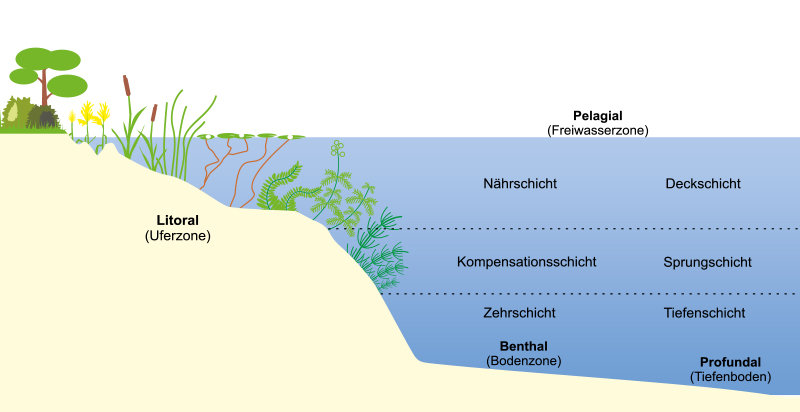
\includegraphics[scale=0.4]{zonierung.jpg}
        \caption{Zonierung des Wassers, Quelle: \cite{klasseWasser}}
        \label{fig:universe}
        \end{figure}
        
    
        Als \textbr{Benthal} bezeichnet man die gesamte Bodenregion in einem stehenden Gewässer. \cite{Was} Sie ist gegliedert in die \textbr{Profundal} und ufernahe \textbr{Litoral}. Letztere ist oberhalb der Kompensationsschicht. Sie ist stark bewachsen von Wasserpflanzen. Hier wird die gesamte organische Masse aufgebaut von der der Teich lebt. Die \textbr{Profundal} befindet sich jedoch unter der Kompensationsschicht und somit findet sich hier kein pflanzliches Leben. \cite{Was} [Seite 36]
    
    \subsection{Nahrungskette, Nahrungsnetz}
    
        Als \citebr{Nahrungskette} bezeichnet man eine graphische Darstellung der Nährstoffübergabe in einem Ökosystem.  Man beginnt hierbei mit einem autotrophen Produzenten, welcher Sonnenlicht in Biomasse umwandelt. Die nächste Stufe ist der Primärkonsument. Dieser ernährt sich heterotroph von dieser Biomasse. Darauf folgen Sekundärkonsument und Tertiärkonsument. \cite{Biobuch} [Seite 318] \\
        \vspace{5mm}
        Da jedoch die meisten Lebewesen von vielen verschiedenen Dingen ernähren, benutzt man ein allgemeineres Modell: Ein \citebr{Nahrungsnetz} verbindet alle Lebewesen in einem Ökosystem durch Ernährungsbeziehungen. Man bezeichnet jetzt nur noch allgemeiner als ``Konsumenten`` und ``Produzenten``, da \textit{die Trophiestufen nicht mehr hierarchisch übereinander sondern ineinander verflochten sind.} \cite{Biobuch} [Seite 319]
    
    \subsection{Stoffkreisläufe}
    
        In den meisten Ökosystemen gibt es zwei parallel laufende \textbr{Stoffkreisläufe}: \\
        \vspace{5mm}
        Der organische Stoffkreislauf besteht aus der Beziehung zwischen den Produzenten, Konsumenten und Destruenten. Konsumenten beziehen ihre Energie aus der Biomasse der Produzenten. Konsumeten wie auch Produzenten sterben ab und werden zuerst zu Detritus. Durch die Destruenten werden sie mineralisiert und in ihre anorganischen Stoffteile zersetzt. Diese können wiederum von den Konsumeten aus dem Boden aufgenommen werden. \cite{Biobuch} [Seite 320] \\
        \vspace{5mm}
        Der anorganische Stoffkreislauf besitzt als Herzstück die Sauerstoff-produzierenden Produzenten. Sowohl Destruenten als auch Konsumenten sind von diesem Sauerstoff abhängig. Als Rückgabe produzieren sie Kohlenstoffdioxid, welcher wiederum von den Konsumenten aufgenommen wird. \cite{Biobuch} [Seite 320] \\


\section{Material und Methoden}
    
    \subsection{Aufspüren und Analyse der Lebewesen im Teich}
    
        % TODO Lu
    
        \begin{table}[h!]
        \centering
        \begin{tabular}{|c|} 
         \hline
         \\
         Planktonnetz, für das Einsammeln von Plankton \\
         kleines grünes Netz, für das Fangen von Insekten, \\ Weichtieren und Amphibien \\
         Konfitüregläser \\
         Pinsel \\
         Pinzette \\
         Pipette \\
         Glasschälchen \\
         Objektträger \\
         Deckgläser \\
         Mikroskop \\
         Binokular \\
         Bestimmungsbuch ``Das Leben im Wassertropfen`` \\ (Strebe et al., Verlag Kosmos, 2002) \\
         Besimmungsbuch ``Was lebt in Tümpel, Bach und Weiher`` \\ (Wolfgang Engelhardt, Verlag Kosmos, 2003) \\[2ex]
         \hline
        \end{tabular}
        \label{Tiere}
        \end{table}
        
        \begin{enumerate}
            \item Netze und Gläser wurden beim Schulteich bereitgelegt.
            \item Es wurde mit dem kleinen grünen Netz nach Insekten, Weichtieren und Amphibien gefischt, indem man im oberen Teich den Untergrund sorgfältig aufwühlte. Gefangene Tiere wurden sachte in die Gläser getan.
            \item Das unten verschlossene Planktonnetz wurde mehrmals durch die unteren Teiche gezogen. Der Fanginhalt wurde in weitere Gläser geleert.
            \item Es wurde auch nach Kleintieren im schlammigen Teil des Gewässers gesucht.
            \item Es wurden einzelne Lebewesen mithilfe der Pipette je nach Grösse entweder in Glasschälchen zu Betrachtung unter dem Binokular respektive auf Objektträger mit Deckgläsern zur Betrachtung unter dem Mikroskop gegeben.
            \item Die Lebewesen wurden vergrössert betrachtet und mit den Bestimmungsbüchern identifiziert. Speziell interessante Fänge wurden ausserdem fotografiert. Alle gefundenen Lebewesen wurden auf der Wandtafel notiert.
            \item Am Ende der Doppelstunde wurden alle Lebewesen zurück in die Teiche gebracht.
        \end{enumerate}
        
    \subsection{Testen der Wasserqualität im Teich}
    
        \begin{table}[h!]
        \centering
        \begin{tabular}{|c|} 
         \hline
         \\
         Schöpfflaschen \\
         pH-Papier \\
         Testkit für Phosphat \\
         Testkit für Nitrit \\
         Testkit für Nitrat \\
         Testkit für Ammonium \\
         Testkit für ph-Wert \\
         Thermometer \\[1ex]
         \hline
        \end{tabular}
        \label{Praktikum1}
        \end{table}
        
        \begin{enumerate}
            \item Wasserproben aus dem Schulteich wurden gesammelt: Zum einem Oberflächenwasser, zum anderen Tiefernwasser. Wasserproben aus grösserer Tiefe liessen sich mit der Schöpfflasche gewinnen. Dazu wurde eine Flasche an einer langen Stange befestigt. Die Flasche wurde auf die gewünschte Wassertiefe gebracht und mit dem Bindfaden der Verschlussstopfen entfernt. Dadurch füllte sich unter Wasser die Flasche. Sobald keine Luftblasen mehr aufstiegen, konnte die Flasche mit dem Tiefenwasser zurückgeholt und mit den Messungen begonnen werden.
            \item Gemäss der Anleitung auf den Testkits wurde eine physikalisch-chemische Wasseruntersuchung durchgeführt. Die Daten wurden festgehalten.
            \item Die Messwerte des Teichwassers wurden mit verdünnten und unverdünnten Dünger verglichen.
        \end{enumerate}
        
        
        \begin{figure}[h!]
        \centering
        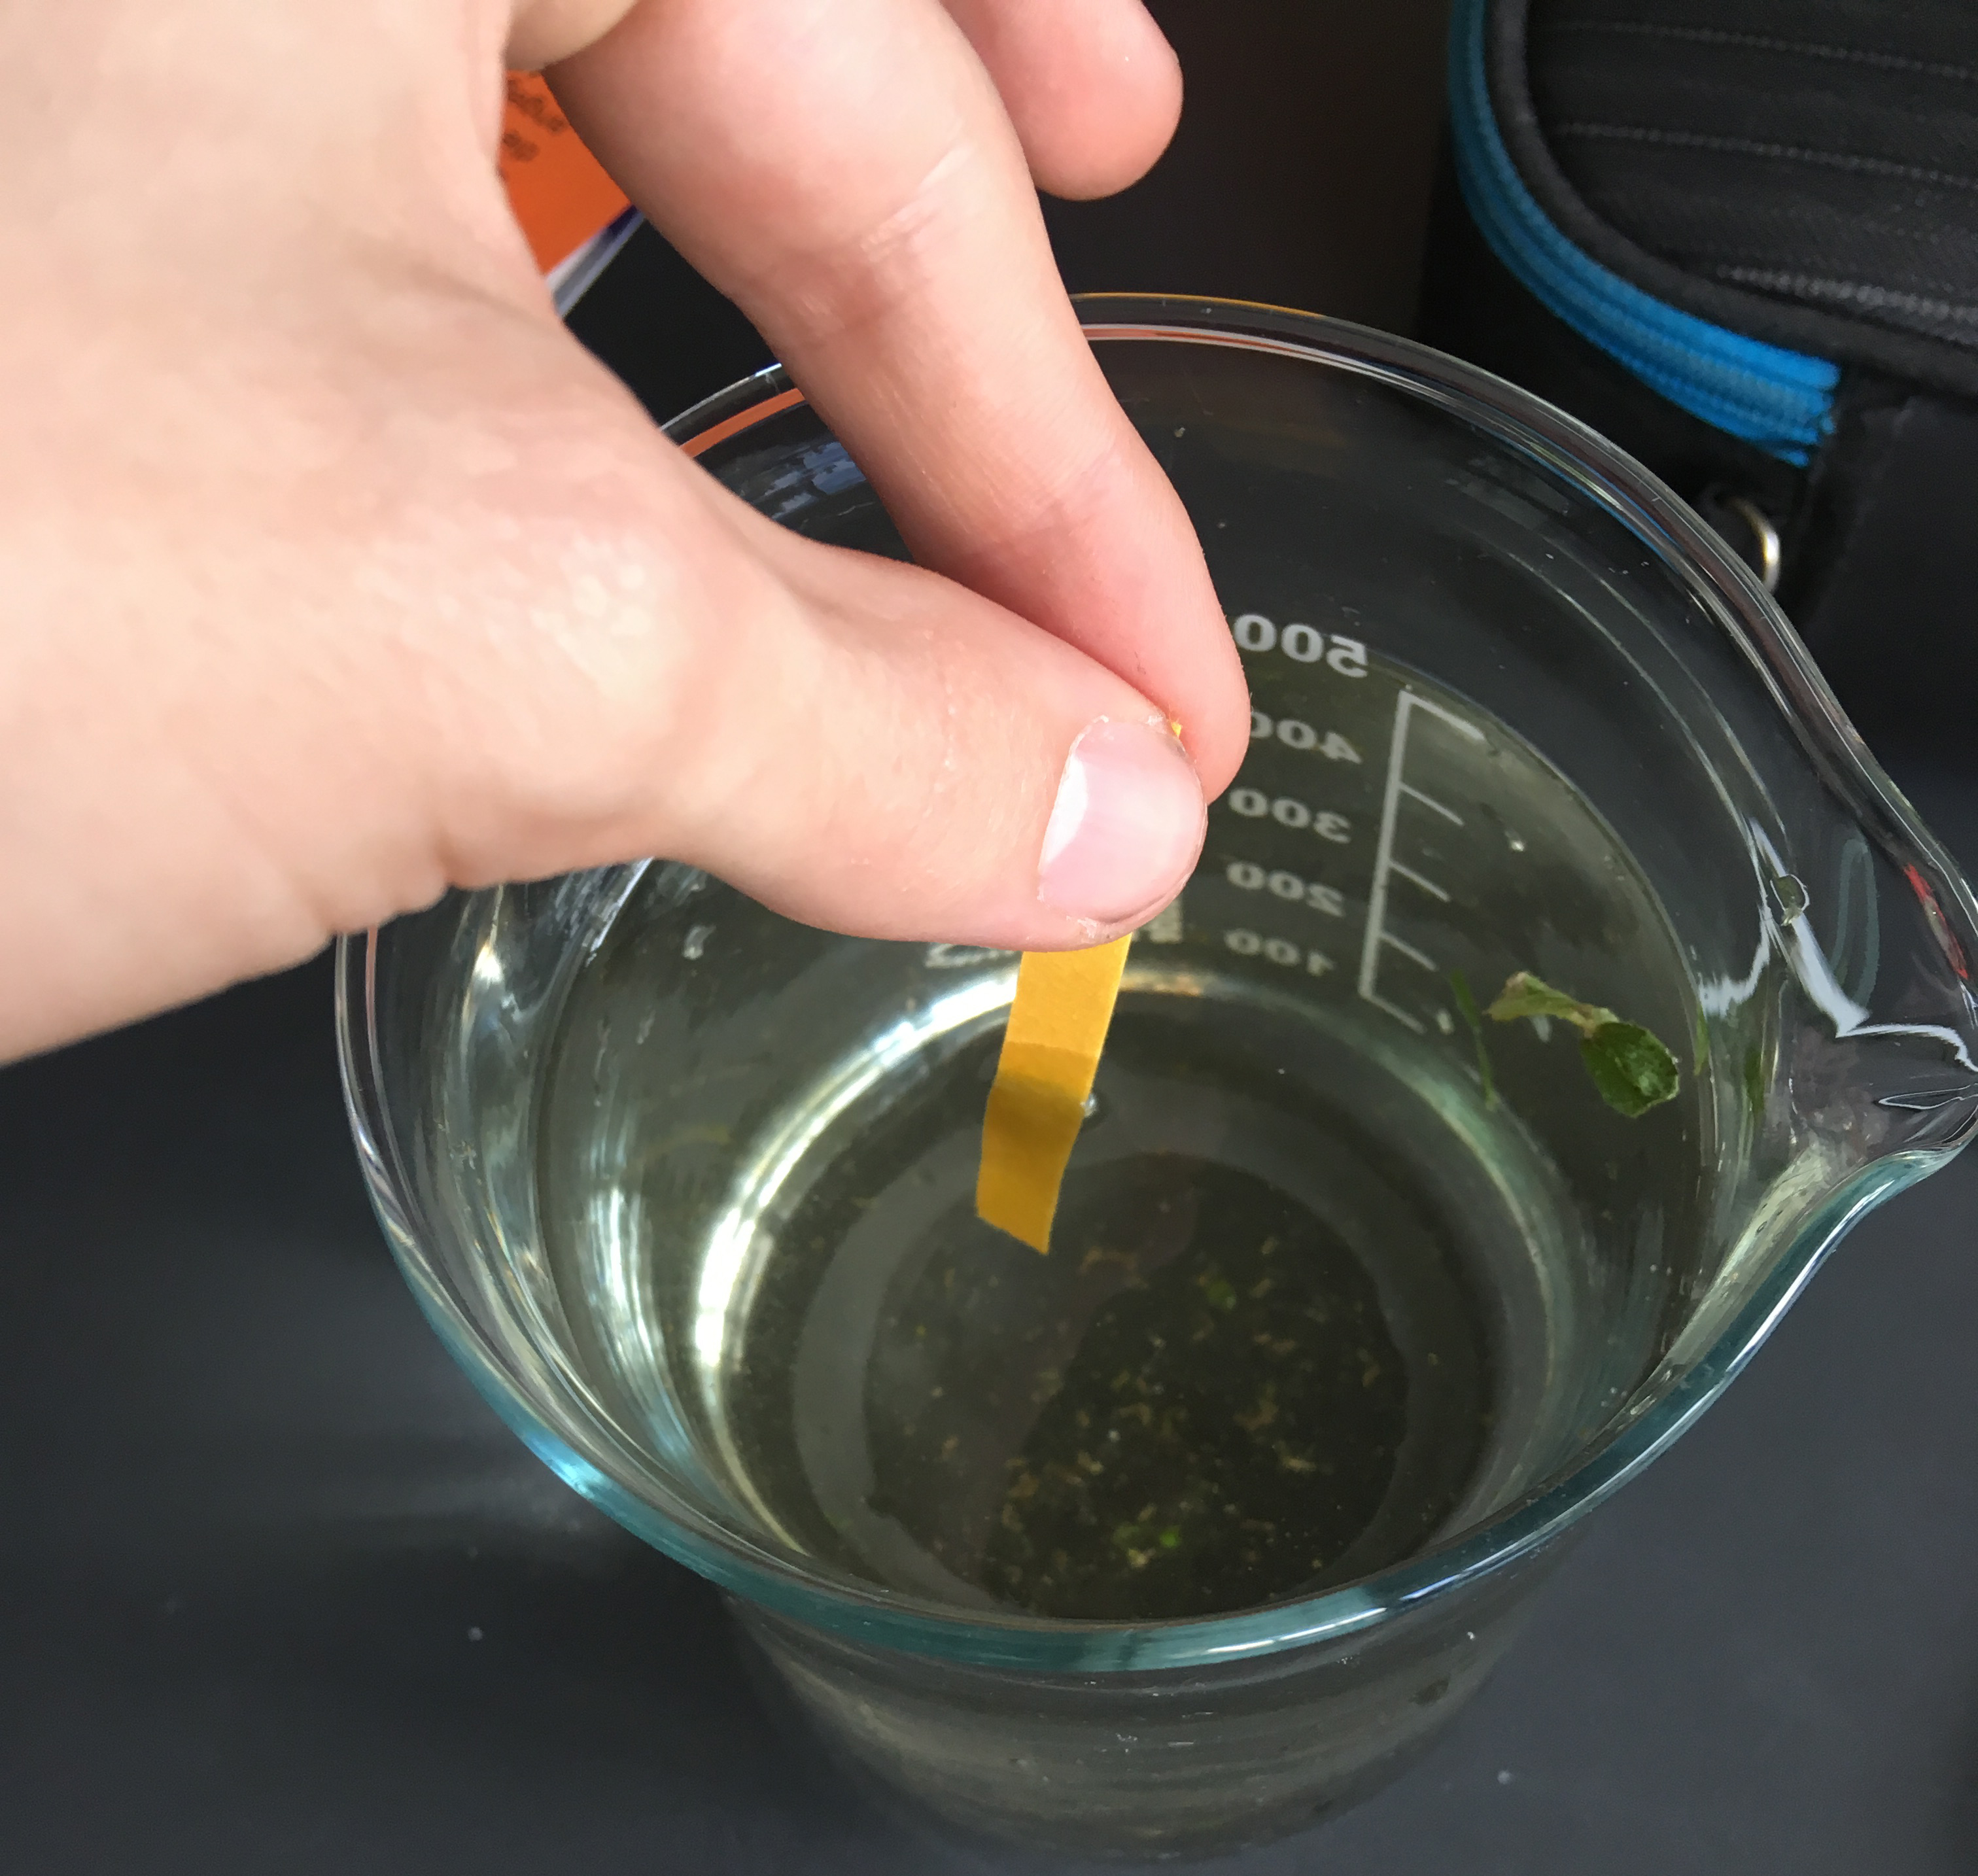
\includegraphics[scale=0.1]{pH-test.jpg}
        \caption{pH-Test}
        \label{fig:universe}
        \end{figure}
        
        \begin{figure}[h!]
        \centering
        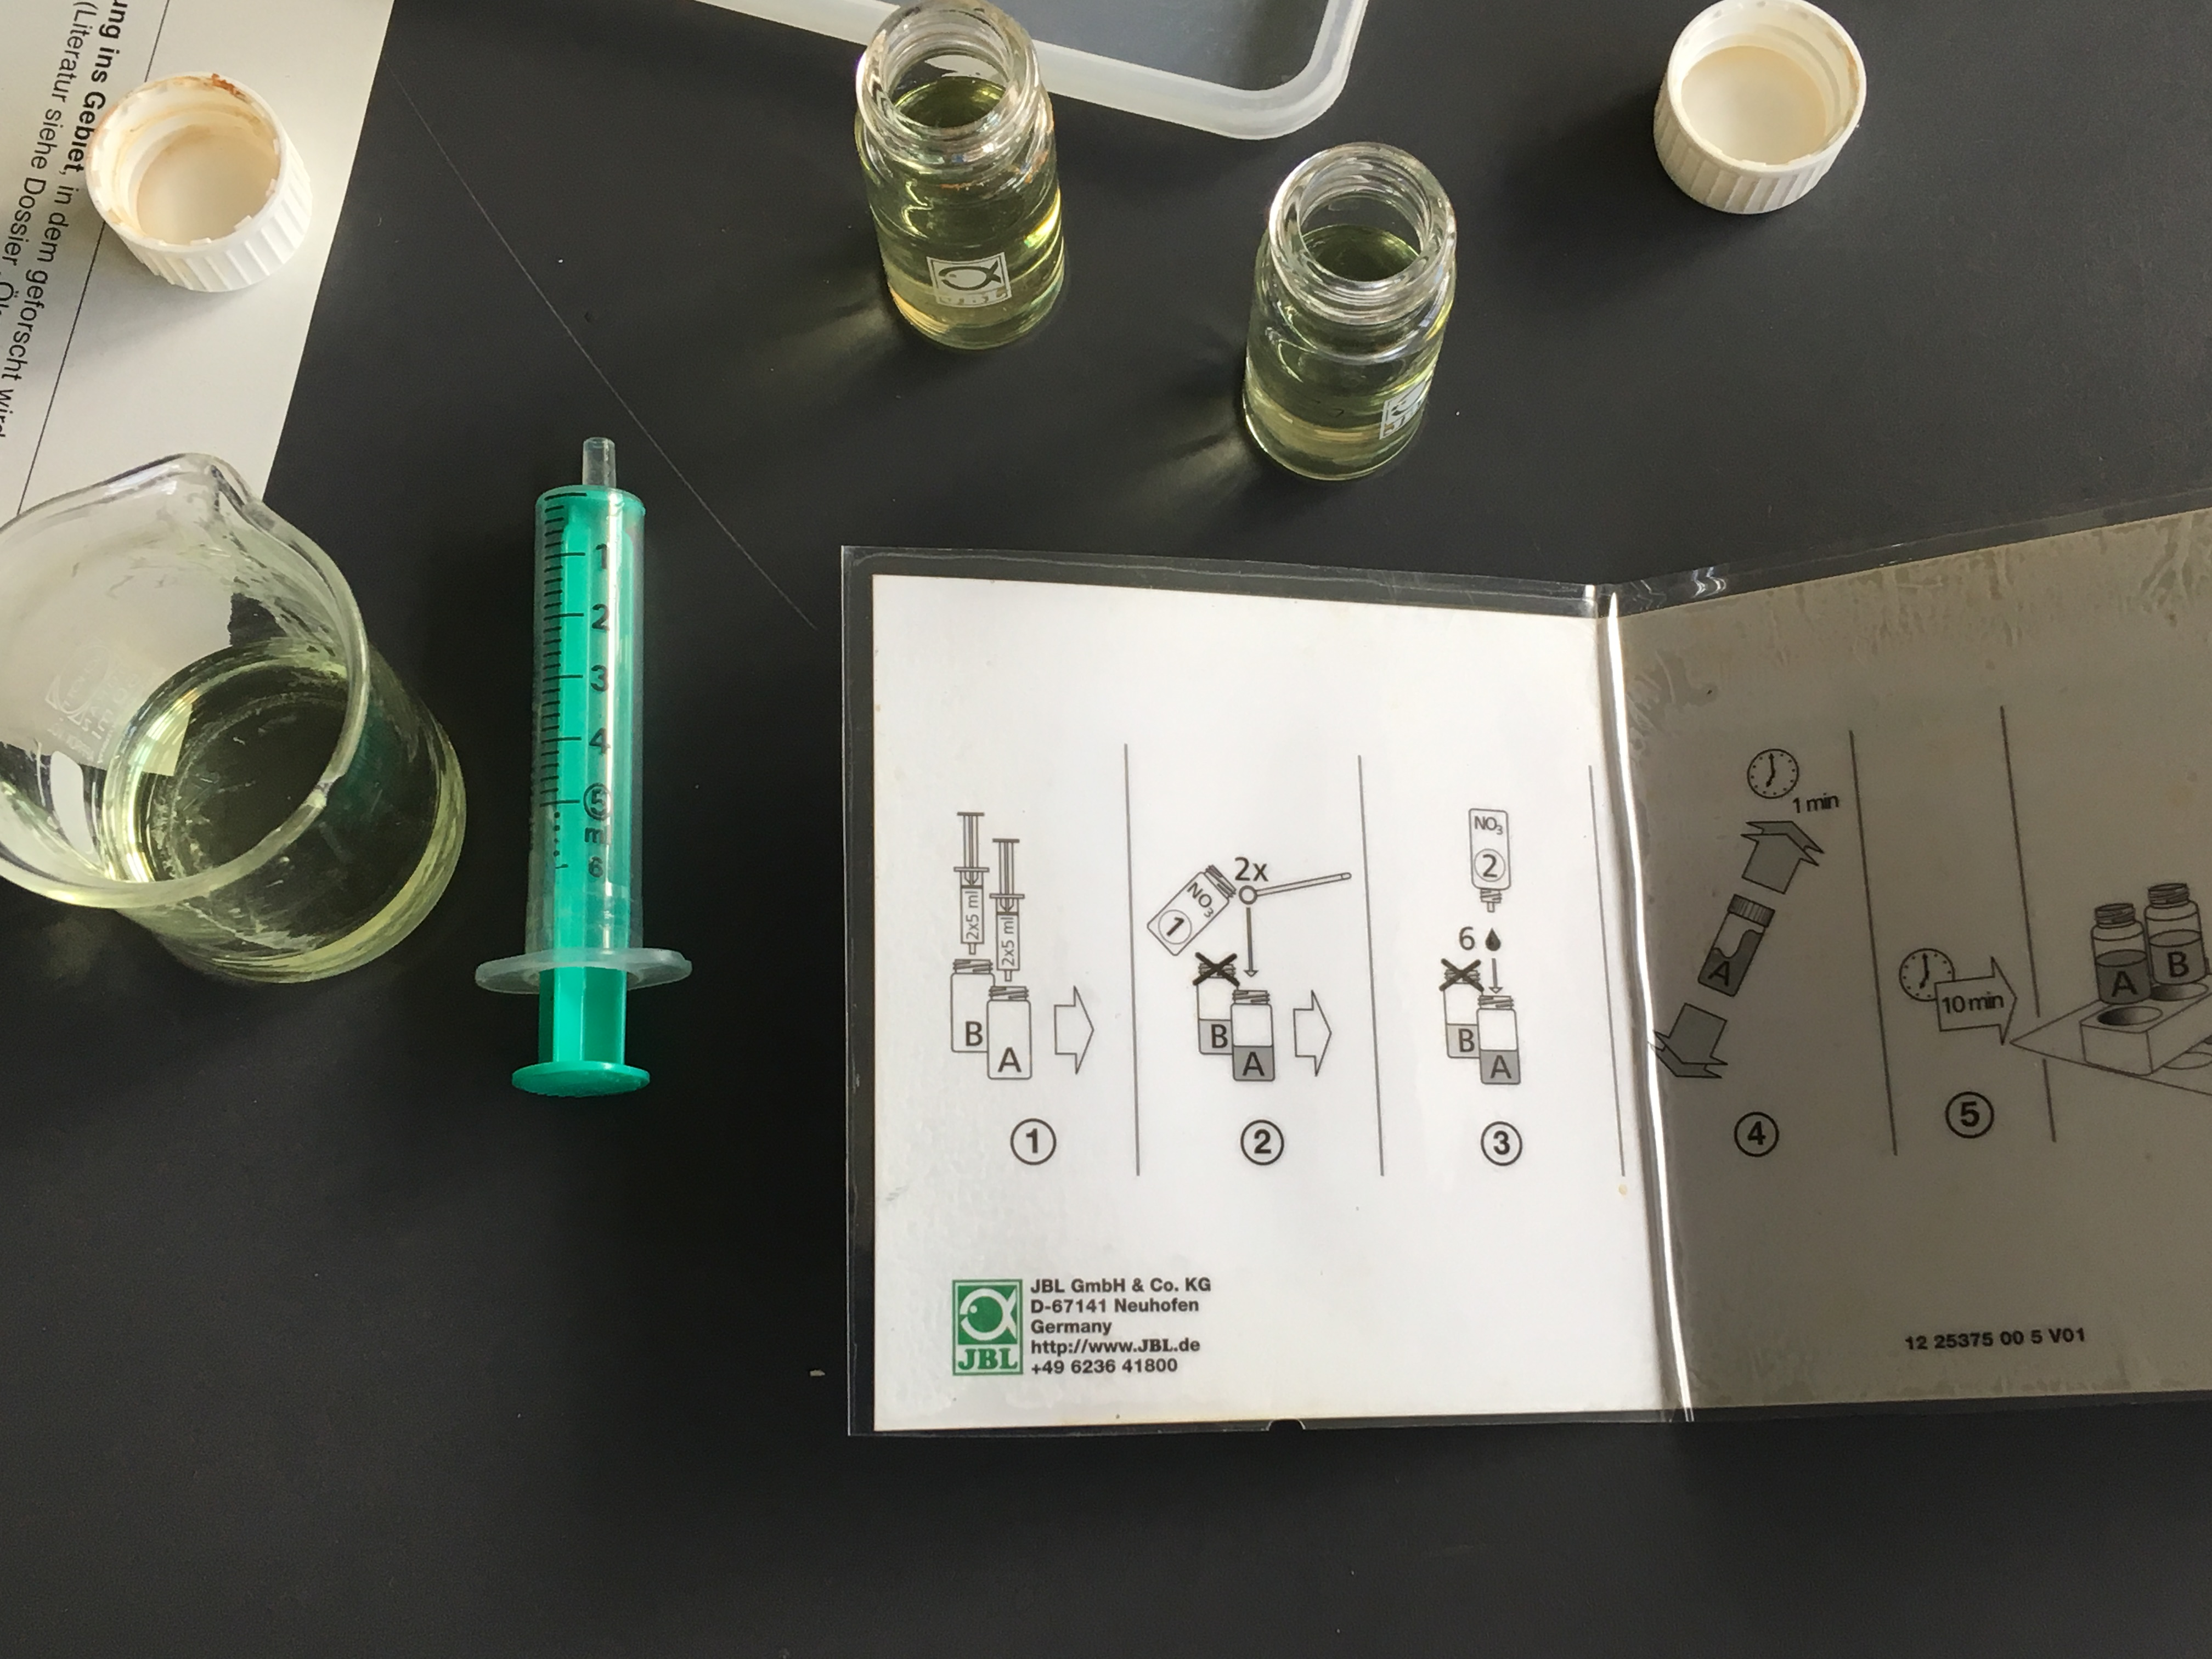
\includegraphics[scale=0.1]{Phosphat-test.JPG}
        \caption{Phosphat-Test}
        \label{fig:universe}
        \end{figure}
        
        \clearpage


\section{Resultate}
    
    \subsection{Nahrungsnetzwerke}
        
        % TODO Bas
    
        \subsubsection{Frühling}
        
        \subsubsection{Frühsommer}
        
    \subsection{Gemessene Wasserwerte}

        n=10
        
        \begin{table}[H]
        \centering
        \caption{Teichwasser:}
        \begin{tabular}{@{}|l|l|lll@{}}
        \cmidrule(r){1-2}
        Temperatur & \begin{tabular}[c]{@{}l@{}}oben: 10℃\\ unten: 9℃\end{tabular} &  &  &  \\ \cmidrule(r){1-2}
        pH-Wert & 7 &  &  &  \\ \cmidrule(r){1-2}
        Phosphatgehalt & 0.05 mg/l &  &  &  \\ \cmidrule(r){1-2}
        Ammoniumgehalt & 0-1 mg/l &  &  &  \\ \cmidrule(r){1-2}
        Nitratgehalt & 2 mg/l &  &  &  \\ \cmidrule(r){1-2}
        Nitritgehalt & 0 mg/l &  &  &  \\ \cmidrule(r){1-2}
        \end{tabular}
        \end{table}
        
        
        
        \begin{table}[H]
        \centering
        \caption{Blumendünger:}
        \label{tab:my-table}
        \begin{tabular}{@{}llllll@{}}
        \toprule
         & Reindünger & n1 & n2 & n3 & n4 \\ \midrule
        pH-Wert & 9 & 8 & 7 & 7 & 7 \\
        Phosphatgehalt & 122 mg/l & \textgreater{}10 mg/l & \textless{}1.8 mg/l &  &  \\
        Ammoniumgehalt &  &  &  & 2 mg/l & 0-1 mg/l \\
        Nitratgehalt & \textgreater{}70 mg/l & 50 mg/l & 10 mg/l & 3 mg/l & 1 mg/l \\
        Nitritgehalt & 0.5 mg/l & 0.35 mg/l & 0 mg/l & 0 mg/l & 0 mg/l \\ \bottomrule
        \end{tabular}
        \end{table}
                        


\section{Diskussion}

    \subsection{Analyse der Nahrungsnetzwerke}
    
        % TODO Bas
        
    % \subsection{Planktonanalyse} potenziell
    
    \subsection{Wasseranalyse}
        
        Werden die Messwerte des Teichwassers betrachtet und mit denen des Blumendüngers verglichen, so erkennt man dass das Teichwasser relativ gesehen doch eher mineralien-arm ist. Das Ökosystem Teich besitzt einen permanenten Stoffkreislauf, bei welchem von Pflanzen Mineralien verbraucht werden und durch Mineralisierung wieder in den Teich hineingeführt werden. Mineralien sind der wichtigste limitierende Faktor für das Pflanzenwachstum, darum führt man diese auch z.B. Blumenbeeten zu. \\
        \vspace{5mm}
        Vor allem im Sommer herrscht ein klares Gleichgewicht, in welchem Pflanzen in der warmen Litoral ganz viel Sauerstoff produzieren, welcher aber nicht in die kalte Benthal gelangt, während in der Bodenzone sich eine grosse Menge an Mineralien ansammelt, der Sauerstoffgehalt aber tief bleibt. \\
        \vspace{5mm}
        Was passiert jetzt aber wenn man Dünger in die mineralien-arme Nährschicht zuführt? \\
        Es ist zu bemerken, dass es sich bei pH um eine Logarithmische Skala handelt, das bedeutet der Unterschied zwischen pH 7 und pH 9 ist nicht 2, sondern ein Faktor von 100. Ein zu basischer pH-Wert ist sehr problematisch für das Ökosystem. Zum Beispiel kann sich Ammonium ($NH_4$) zu giftigem Ammoniak ($NH_3$) umwandeln.\cite{Teichpflege} Noch viel schlimmer sind aber die einzelnen Mineralien und zwar auf eine sehr paradoxe Weise: Sie beschleunigen den Pflanzenwachstum \\
        \vspace{5mm}
        Hier wird von Überdüngung gesprochen. Wird nun der pflanzen-reichem, mineralien-armen Litoral Dünger zugeführt, so wird das sensible Gleichgewicht gestört. Zuerst profitieren alle: Die Pflanzen wachsen und die Tiere ernähren sich vom den neuen Produzenten. Doch bald wird der Pflanzen- und vor allem Algenteneppich an der Wasseroberfläche so dicht, dass kein Sonnenlicht mehr in alle tieferen Zonen der Litoral dringt. Was folgt ist ein Aussterben einer extremen Menge an 
        \vspace{5mm}
        Bei so viel Detritus vermehren sich die Destruenten stark. Dabei wird sehr viel Sauerstoff verbraucht. Jetzt kippt der Teich: Die meisten Sauerstoff-Produzenten sind gestorben, es gibt ganz viele neue Sauerstoff-verbraucher. Die Sauerstoffkonzentration im Biotop sinkt was zu einem Massensterben führt. Produzenten, Konsumenten und Destruenten sterben aus. Das Ökosystem ist tot. \cite{Planet1} \cite{Planet2} \\
        \vspace{5mm}
        Die tiefe Mineralien-Menge des Teiches ist notwendig für das Überleben des Ökosystems. Mineralien sind zwar unabdingbar für Pflanzenwachstum, doch sind Düngungsmittel lebensgefährlich für das Leben im Teich. Industrie und Landwirtschaftsabfälle sollten und dürfen nicht einfach in Teiche und Seen gelangen. \cite{Tagi} Selbst ein Verhältnis von 1:1000 (Ergebnisse n3) zwischen Dünger und Wasser besitzt noch gefährliche Mengen an Mineralien. \\
       
    \section{Danksagung}

    Vielen Dank an alle Fotografen, inklusive Cino, Fatima und Lisa für die Hilfe beim Zusammenstellen der Bilddatenbank dieser beiden Biopraktiken.



    \begin{thebibliography}{9}
    \centering{
        \bibitem{Biobuch}
       Dr. Jürgen Braun, Heinrich Joussen, Dr. Andreas Paul, Elsbeth Westendorf-Bröring: Biologie Heute erweiterte Ausgabe \textit{Schroedel Westermann, 2002}
        \bibitem{Biologie-schule.de}
        Website: \textit{http://www.biologie-schule.de/oekosystem.php} \\ 23.5.19
        \bibitem{Duden}
        Website: \textit{https://www.duden.de/rechtschreibung/} \\ 23.5.19
        \bibitem{Kleingewasserkunde}
        Dieter Glandt: Praktische Kleingewässerkunde \textit{Laurenti Verlag, Bielefeld 2006} \\ \textit{Gefunden über Wikipedia}
        \bibitem{Spektrum}
        Website: \textit{https://www.spektrum.de/lexikon/biologie/} \\ 23.5.19
        \bibitem{EvolutionofInsects}
         David Grimaldi, Michael S. Engel: Evolution of the Insects. (= Cambridge Evolution Series).  \textit{Cambridge University Press, 2005} \\ 
         \textit{Gefunden über Wikipedia} \\
         \bibitem{FrustfreiLernen}
        Website: \textit{https://www.frustfrei-lernen.de/biologie/wirbeltiere-wirbellose-tiere-biologie.html} \\  23.5.19
        \bibitem{UniProtokolle}
        Website: \textit{http://www.uni-protokolle.de/Lexikon/Taxon.html} \\ 23.5.19
        \bibitem{Lernhelfer}
        Website: \textit{https://www.lernhelfer.de/schuelerlexikon/biologie/artikel/wirbeltiere} \\ 23.5.19
        \bibitem{Lupos}
        Website: \textit{http://www.lupos-landleben.de/wasserpflanzen-im-teich/} \\ 24.5.19
        \bibitem{klasseWasser}
        Website: \textit{https://www.klassewasser.de/content/language1/html/6148.php} \\ 24.5.19
        \bibitem{Was}
        Wolfgang Engelhardt: Was lebt in Tümpel, Bach und Weiher \textit{Verlag Kosmos, 2003} \\
        \bibitem{Teichpflege}
        Website: \textit{https://www.teichpflege.eu/bauanleitungen/die-richtigen-wasserwerte/ph-wert/} \\ 31.5.19
        \bibitem{Planet1}
        Website: \textit{https://www.planet-schule.de/wissenspool/lebensraeume-im-see/inhalt/hintergrund/kreislaeufe-im-see/was-passiert-bei-ueberduengung.html} \\ 31.5.19
        \bibitem{Planet2}
        Website: \textit{https://www.planet-schule.de/sf/multimedia-interaktive-animationen-detail.php?projekt=gewaesser-ueberduengung} \\ 31.5.19
        \bibitem{Tagi}
        Website: \textit{https://www.tagesanzeiger.ch/schweiz/baldeggersee-ist-wegen-landwirtschaft-ueberduengt/story/20722296} \\ 31.5.19
        
        
        
    }
    \end{thebibliography}

\end{document}
